\Chapter{RESEARCH GENERAL WORKFLOW}\label{sec:Theme1}



As stated in \autoref{sec:Introduction}, the goal of our research project is to create an expertise model based on a series of metrics mined from the Linux Git repository and various mailing lists.






This masters research project consisted of two different parallel projects. On one hand, in a collaboration with the linux foundation, we created and open-sourced 2 tools: Srcmap and Email2git. On the other hand, we created and evaluated an expertise detection model, which was submitted as a paper to the IEEE International Conference on Software Analysis, Evolution and Reengineering\footnote{\url{http://saner.unimol.it/}}. This chapter will discuss the details of both side of the research project, and the links between them.


\section{Srcmap}

In the interest of offering more visibility to the authors of the Linux Kernel, we built a data visualization tool capable of displaying a wide array of information about directories or files found in the linux git repository. We wanted to display the following data points about each file and directory of the source code:

\begin{itemize}
	\item \ac{LOC}
	\item Median age of the \ac{LOC} within a file/directory
	\item Number of lines of code modified since 2016
	\item A list of the 20 developers with the most lines of code
	\item A bar plot displaying the distribution of line of code age
\end{itemize}

We needed an interface that would allow the user to navigate the different files and direcotries of Linux while displaying our list of datapoints, which is why we chose to base the tool on a treemap. Treemaps, which were introduced by Shneiderman~\citep{Bederson-2002} as a solution to display large hierarchical dataset on a 2 dimentional plane, were a great fit for our tool's requierments. 

\subsection{Srcmap 1.0}

In the first version of Srcmap\footnote{\url{http://mcis.polymtl.ca/~courouble/linux.html}}, we used the Google Chart treemap implementation\footnote{\url{https://developers.google.com/chart/interactive/docs/gallery/treemap}}. This easy to use library allowed us to create a quick proof of concept. 

\begin{figure}[htb]
\centering
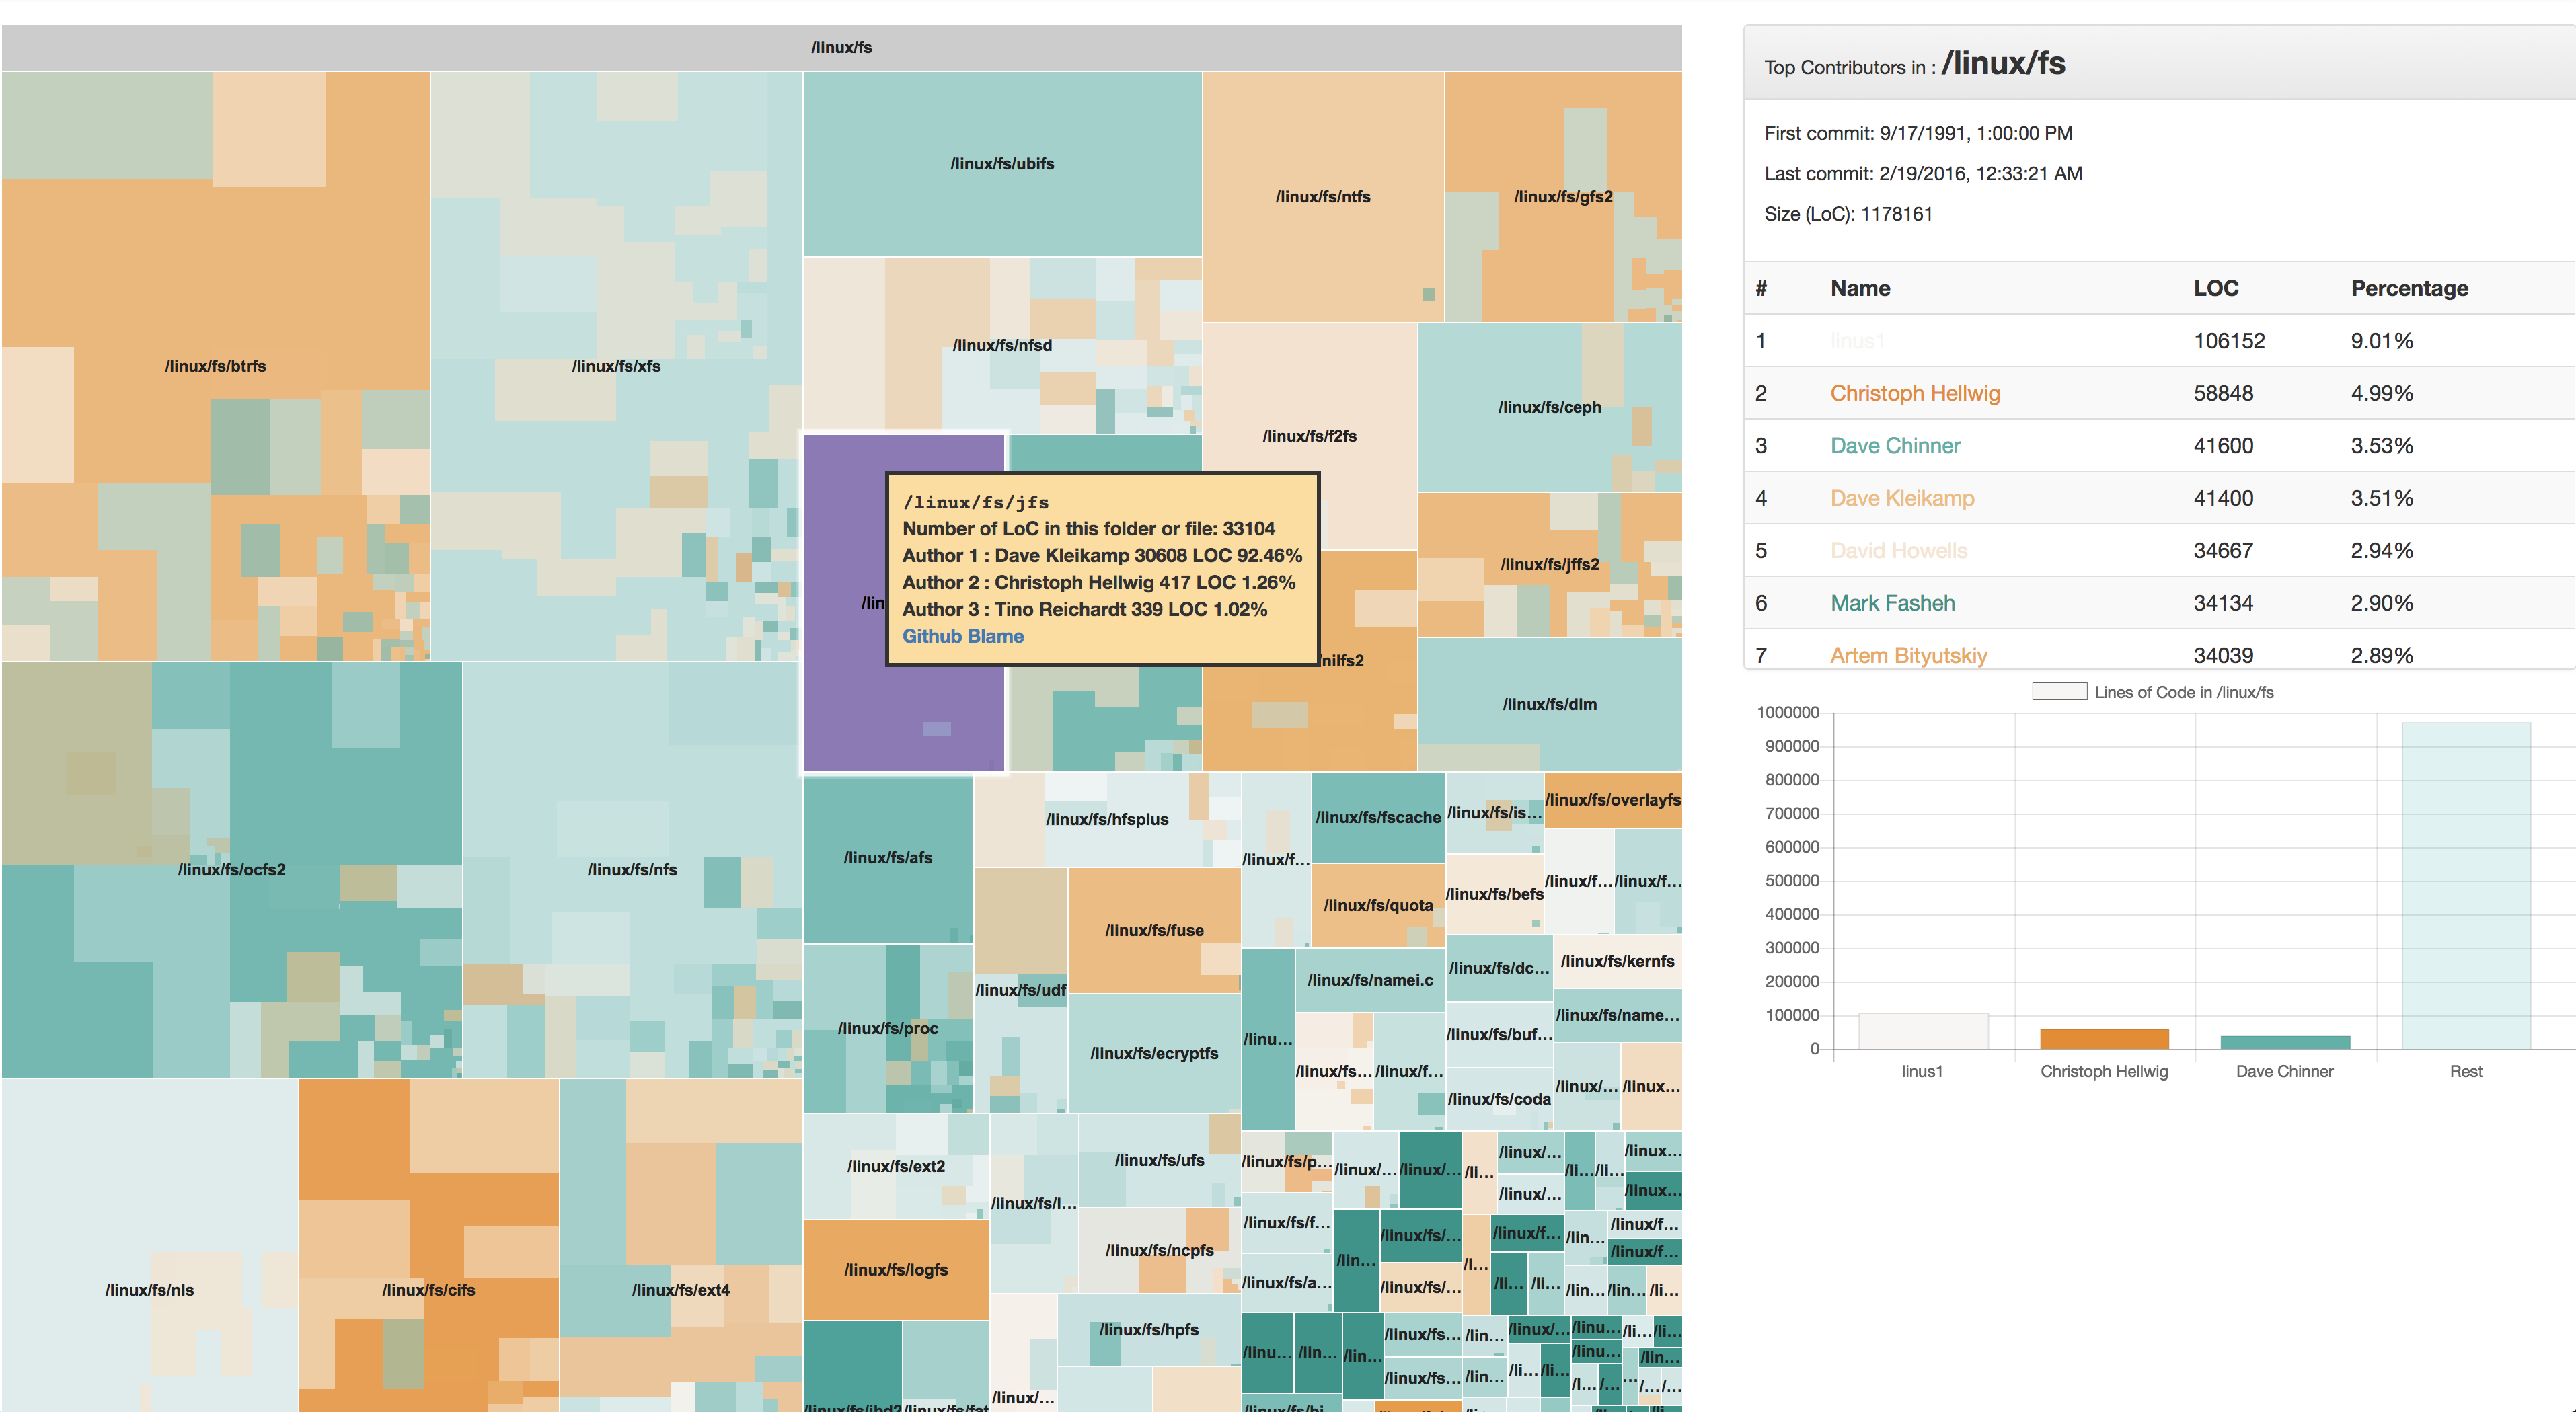
\includegraphics[width=5in]{srcmap1}
\caption{First version of srcmap}
\label{fig:srcmap1}
\end{figure}

\autoref{fig:srcmap1} shows the first version of Srcmap. The diferent boxes represent subdirectories of the Linux Kernel. The different colors present within each box give a preview of the content of the box. In this version of the tool, the color represents the developer having contributed the most lines of code in the contained files. Furthermore, the size of the boxes is proportional to the number of lines of code existing within the file or directory represented by the box. The panel on the right of the screen and the tooltip contain most of the data: exact number of lines of code, age of the first and last lines of code to be added, and the top 20 authors and their percentage of lines of code contributed.

Even though the library offered by Google allowed us to quickly provide a strong proof of concept, we discovered some limitations when we tried adding new features to the tool. The tool had issues handling the size of the dataset. The actual data would take up to 30 seconds to load, and navigating between each node became very slow. This is why we decided to create a new version of the tool with a different treemap library.


\subsection{Srcmap 2.0}


After some research, we discovered a new treemap implementation\footnote{\url{https://carrotsearch.com/foamtree/}} capable of handling large dataset and deeply nested stuctures, which we used for the second version of the tool\footnote{\url{http://mcis.polymtl.ca/~courouble/dev/}}. This new version, shown in \autoref{fig:srcmap2}, introduced three important features: 
\begin{itemize}
	\item Coloring the files and directories according to three metrics:
	\begin{itemize}
		\item \ac{LOC}
		\item Median age
		\item Number of commits since 2016, or "Hot files"
	\end{itemize}
	\item File search
	\item A plot displaying the \textit{age} distribution of \ac{LOC} present in the file/directory.
\end{itemize}

\begin{figure}[htb]
\centering
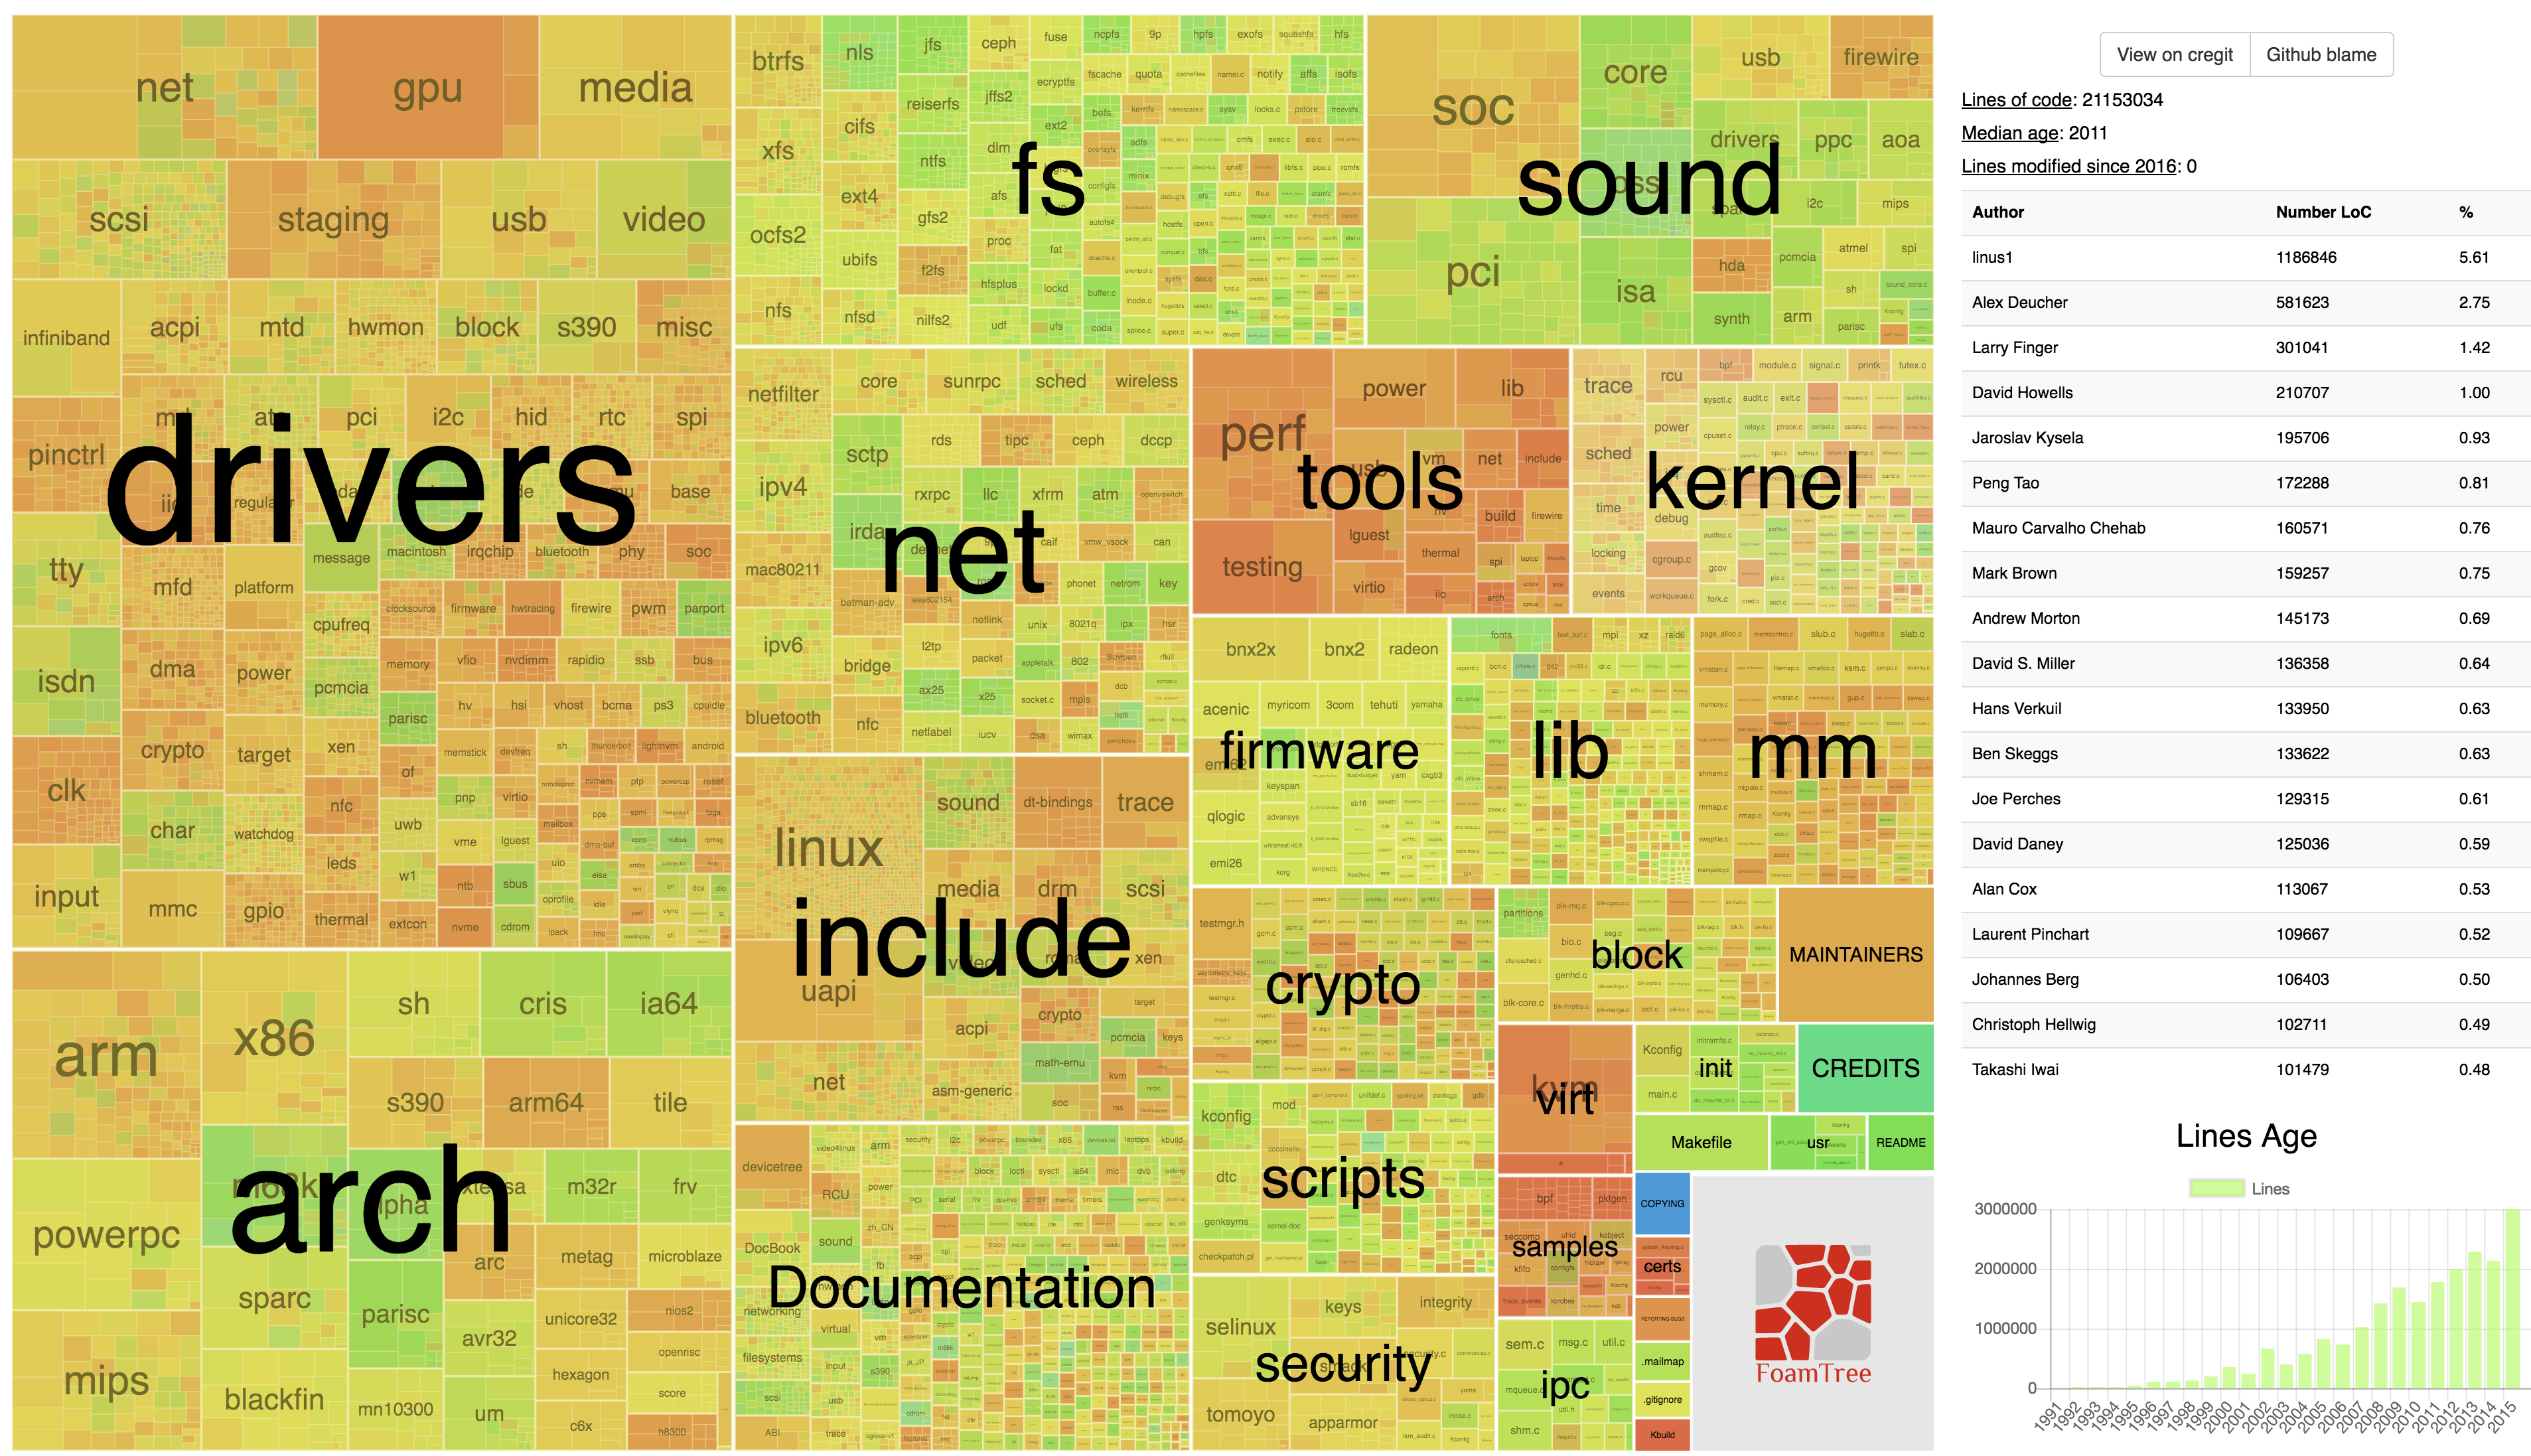
\includegraphics[width=5in]{srcmap2}
\caption{Second version of srcmap}
\label{fig:srcmap2}
\end{figure}

Although the foamtree library had a steeper learning curve than the Google Charts Treemap library, the versatility provided by the foamtree library allow us to provide a much more pleasant user experience and easier access to the data.

I was given the oportunity to travel to Santa Fe, New Mexico to present Srcmap and Cregit at the Linux Plumbers Conference. After discussing srcmap and my research to a series of linux developers, it became evident that there was real interest for another aspect of linux development: linking Linux git commits to email patches and code reviews.


\subsection{Scalability}

\subsection{Community Engagment}

\subsection{Lessons Learned}


\section{Email2git}

The linux contribution process has been a reliable way to pipe code contributions (patches) from developers around the world, to the main Linux repository. With a working copy of the Linux Kernel on their computers, developer can modify the source code and, if desired, submit their changes for review, in hope to integrate the main tree. These changes are submitted as patches, files that contain the lines that are to be removed and the lines that are to be added. To submit a patch, developer send the patch file(s) to a linux maintainer in an \textit{email} with a description of the changes brought by the patch. If accepted, the maintainer will \textit{commit} the changes to his local git repository, and submit the changes \textit{upstream} to another maintainer. 

Although this system has been very reliable, it has one major drawback: once committed, it is impossible to easily find the email conversation that eventually led to the creation of the patch. We addressed this drawback by creating an algorithm capable of backtracking the origin of commits in the Linux Git repository. The algorithm is described in chapter 4.

The data generated by the algorithm consists of a list of commit to patch matches. The matches are accessible online through two interfaces: as a commit ID search through the Email2git interface\footnote{\url{http://mcis.polymtl.ca/~courouble/email2git/}}, or though the Cregit interface\footnote{\url{https://cregit.linuxsources.org/}}.

\subsection{Scalability}

\subsection{Community Engagment}

\subsection{Lessons Learned}




\section{Integrating Email2git with Cregit}

Cregit is a project that aim at providing a finer grain approach to \textit{git blame}. The blame option in git returns the name of the developer who last changed a line of code in the source code. It provides a great way to quickly unmask the developers responsible for code in the Source Code. However, it has a serious limitation: git blame assigns a line to a developer even after a small modification to that line. For instance, if developer $A$ writes \texttt{print "Hello world"}, this line will then become associated with developer $A$. However, if developer $B$ modifies the line to read \texttt{print "Hello world!"}, git blame will associate the line with devloper $B$ even though developer $B$ only added a character. 

Cregit addresses this limitation by tokenizing the source code in a git repository to enables git blame at a token level, instead of a line level. This provides a better understanding of the true authors of the source code. A tokensize version of the Linux kernel source code is available online through the cregit interface\footnote{\url{https://cregit.linuxsources.org/}}.

\begin{figure}[htb]
\centering
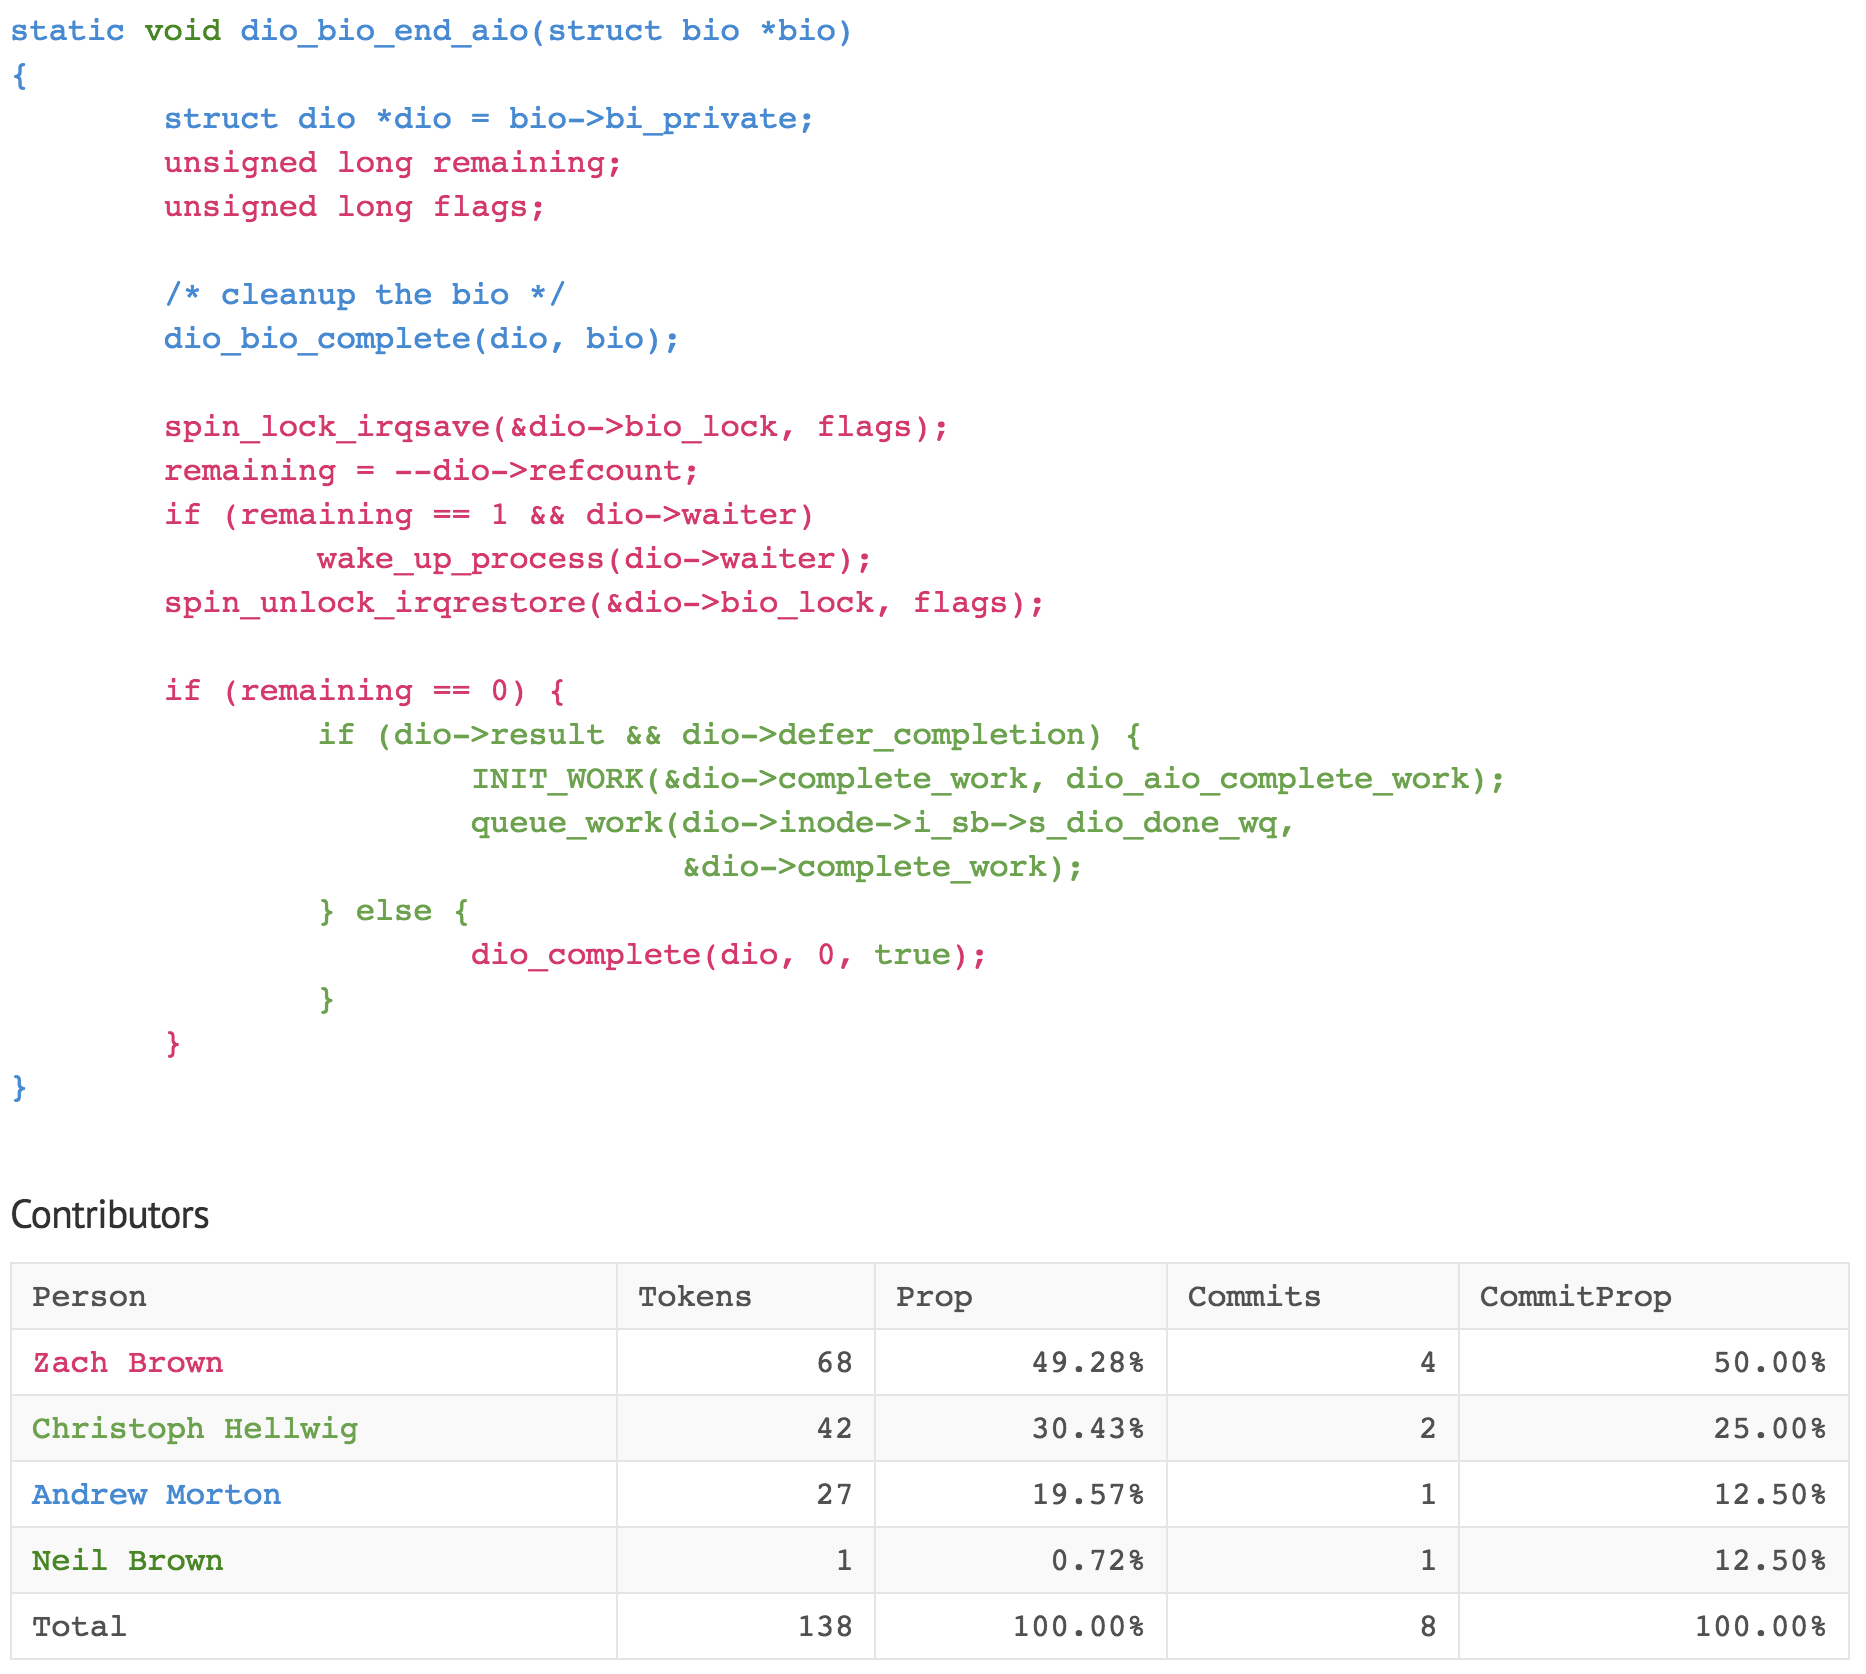
\includegraphics[width=3.5in]{cregit_code}
\caption{Tokenized source code as it appears on Cregit.}
\label{fig:cregit_code}
\end{figure}

\autoref{fig:cregit_code} shows tokenized linux code as it appears on the Cregit interface. In an effort to ease the access to email2git data, we decided to provide access to the matches through cregit. To this end, I modified the user interface to display a window containing all the available patches after clicking on a token, as shown in \autoref{fig:cregit_matches}. 

\begin{figure}[htb]
\centering
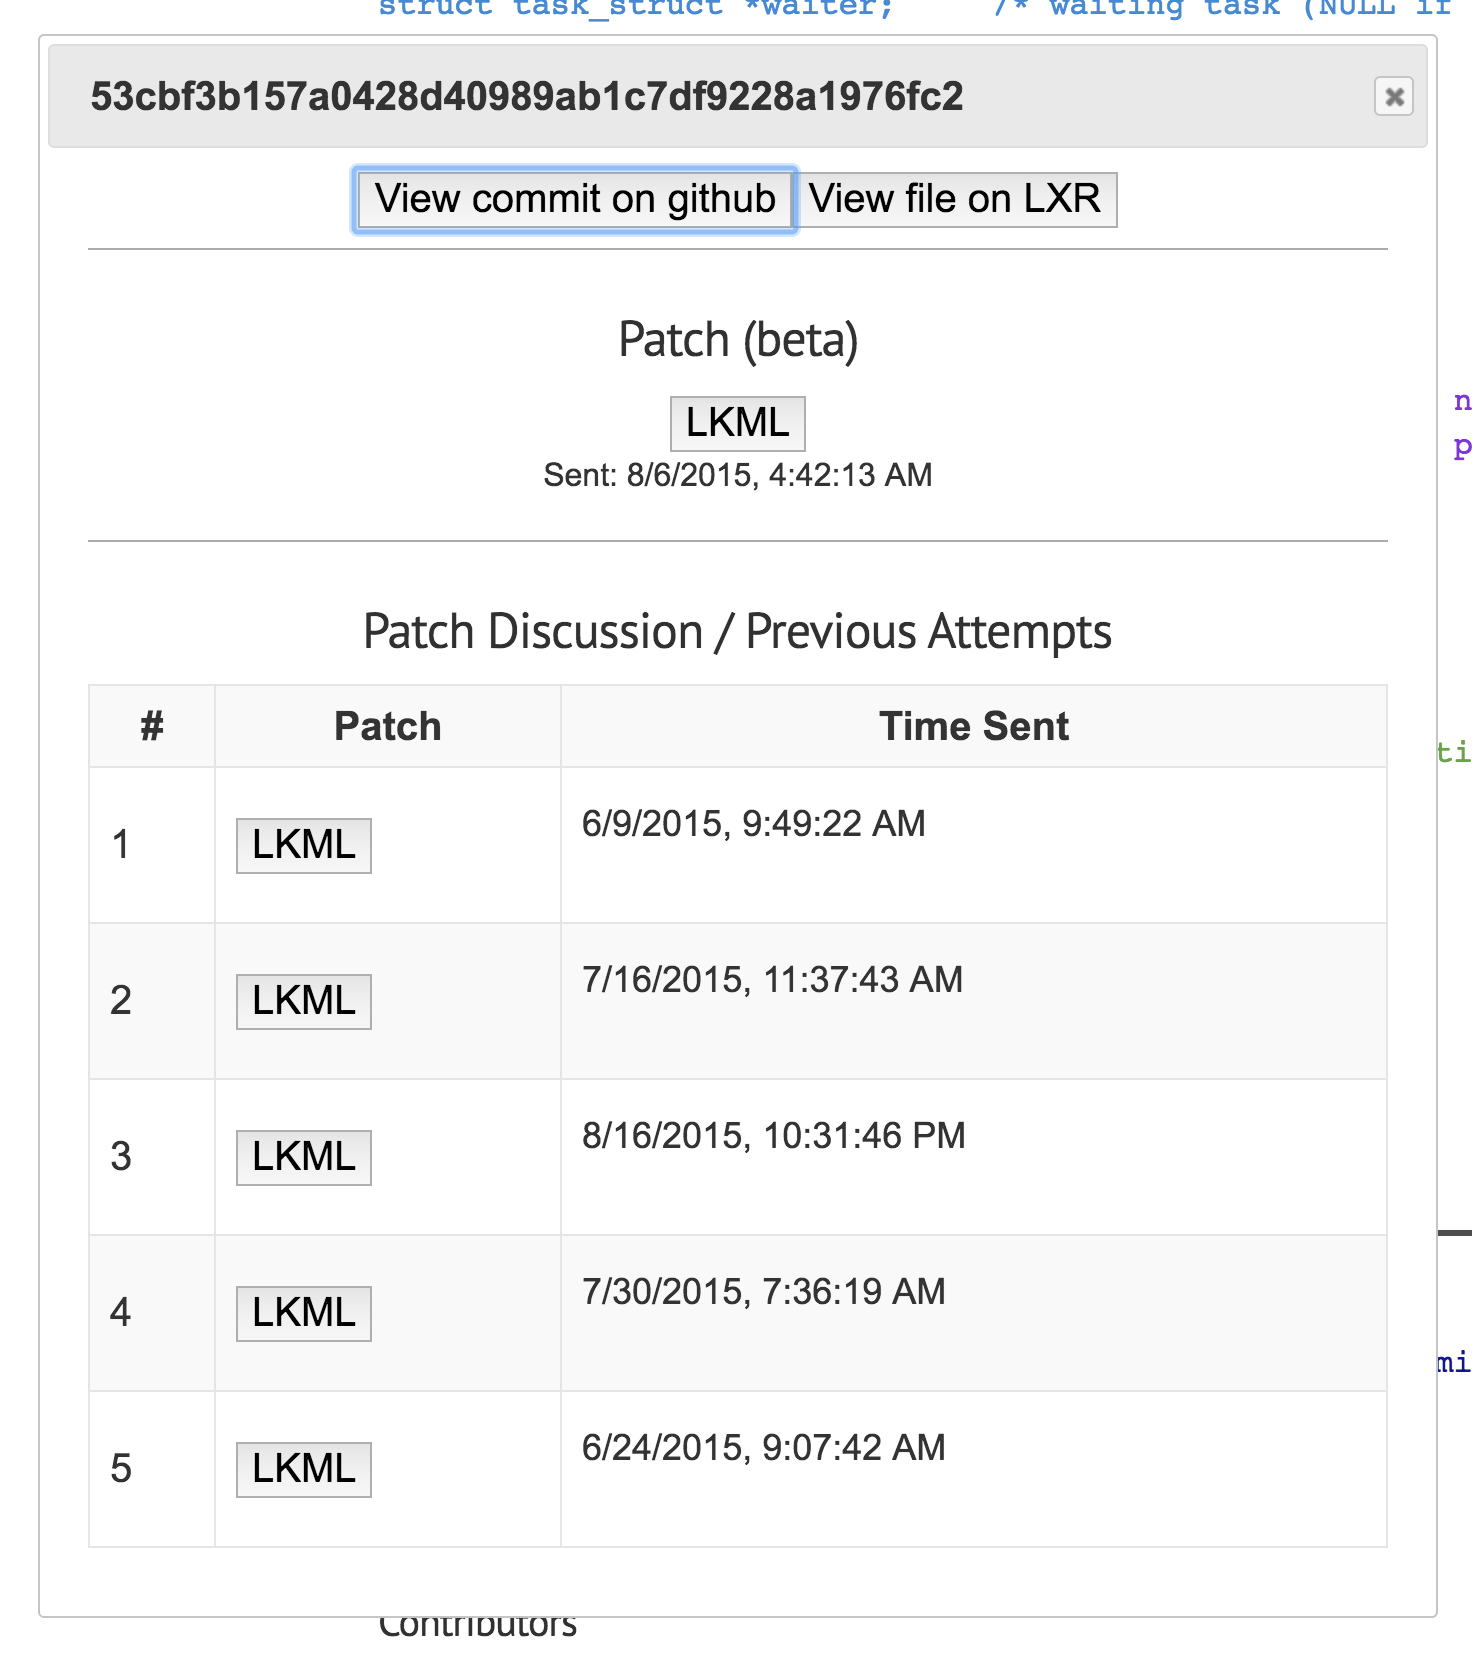
\includegraphics[width=3.5in]{cregit_matches}
\caption{Window containing the patches that introduced the commit associated with the clicked token}
\label{fig:cregit_matches}
\end{figure}



\section{Recommendations}

